\documentclass[fr]{../../../../../../eplexam}
\usepackage{mhchem}
\usepackage{enumitem}
\usepackage[alsoload=synchem, binary-units=true]{siunitx}

\hypertitle{Chimie}{3}{EPL}{1302}{2020}{Janvier}{All}
{Baptiste Laterre}
{Hervé Jeanmart et Joris Proost}

\section{Question 1 : RedOx}

La pile à combustible est un procédé faisant intervenir 2 réactions en milieu alcalin : l’oxydation de \ce{H2_{(g)}} et la réduction de l’\ce{O2_{(g)}} de l’air ambiant. Voici une représentation de la situation étudiée :
\begin{figure}[h]
    \centering
    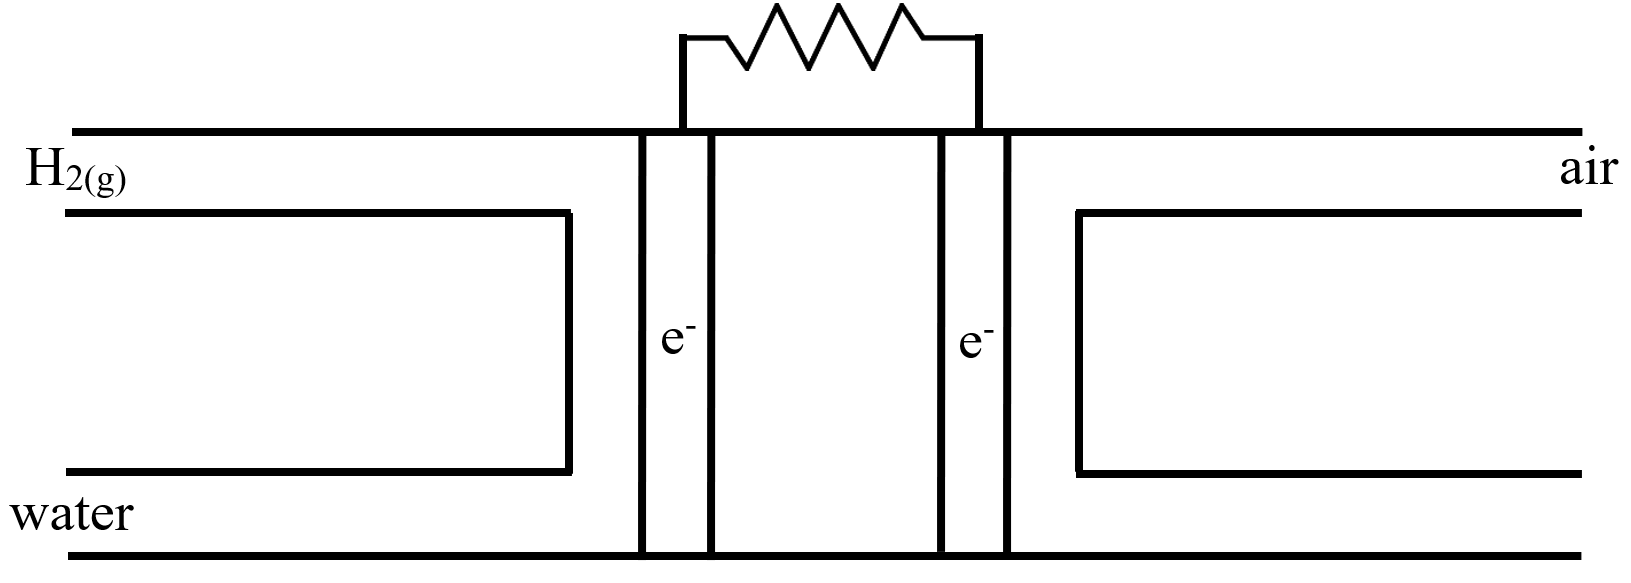
\includegraphics[scale=0.25]{pile_combustible.png}
    \caption{Q1}
    \label{fig:my_label}
\end{figure}

\begin{enumerate}
    \item Ecrivez les 2 demi-réactions ainsi que la réaction globale.
    \item Sur le schéma, indiquez l’emplacement de la cathode, de l’anode, le sens des ions hydroxyde et le sens des électrons.
    \item Trouvez le potentiel d’équilibre de chaque demi-réaction.
    \begin{tabular}{|c|c|c|}
    \hline
    & \ce{H2O} & \ce{OH-} \\
    \hline
    ${\Delta}_fG^o$ (\si{kJ/mol}) & -273.18 & -157.28\\
    \hline
    \end{tabular}
    \item Trouvez la force électromotrice standard. Le pH influence-t-il la force électromotrice ?
\end{enumerate}

\nosolution

\section{Question 2 : cinétique}

Voir Question 1 Septembre 2016.

\begin{solution}
Voir Solution Question 1 Septembre 2016
\end{solution}

\section{Question 3 : cycle}

Ci-après se trouvent les 5 étapes d’un cycle en système fermé.
\begin{itemize}
    \item 1-2 : compression suivant la relation $pV^k$ = cste
    \item 2-3 : réchauffement isochore
    \item 3-4 : réchauffement isobare
    \item 4-5 : détente adiabatique
    \item 5-1 : refroidissement isochore
\end{itemize}
Pour ce cycle, le rapport de compression de $V_\text{max}/V_\text{min}=12$;
la température max est de \SI{1600}{\celsius};
la pression max est de \SI{160}{\bar};
le gaz est comparable à de l’air pour lequel $\lambda = 1.3$;
l’apport de chaleur en 2-3 vaut \SI{1000}{kJ/kg};
l’apport de chaleur en 3-4 vaut \SI{500}{kJ/kg};
le refroidissement en 5-1 fait perdre \SI{600}{kJ/kg}.
À partir de ces données, trouvez les éléments suivants, en indiquant l’ordre dans lequel vous les avez trouvé :

\begin{center}
\begin{tabular}{|m{1cm}|m{9cm}|m{2cm}|}
\hline
    & Valeur de $k$ (transformation 1-2) & \\
    \hline
    & Pression à l’état 2 (\si{bar}) & \\
    \hline
    & Pression à l’état 5 (\si{bar}) & \\
    \hline
    & Variation d’énergie interne entre 1 et 2 (\si{J}) & \\
    \hline
    & Sachant que le travail total du cycle est de \SI{-1000}{J},
    trouvez la masse de gaz dans le système (\si{kg}) & \\
    \hline
    & La température à l’état 3 (\si{K}) & \\
    \hline
\end{tabular}
\end{center}
Tracez également les diagrammes p/V et S/T pour ce cycle.

\nosolution

\section{Question 4 : théorie}

Dans le cadre du premier principe, nous avons défini $\pi_T$ et $ \mu_{J-T}$.
\begin{enumerate}
    \item Donnez une définition mathématique de $\pi_T$.
    \item Par quelle réalité physique ce coefficient ne peut être nul ?
    \item En utilisant le schéma ci-dessous, expliquez une expérience qui illustre l’effet Joule-Thomson.
    %\begin{figure}
    %   \centering
    %    \includegraphics{}
    %    \caption{Caption}
    %    \label{fig:my_label}
    %\end{figure}
    \item En se référant à l’expérience précédente, l’entropie du gaz change-t-elle au cours de la réaction ?
\end{enumerate}

\nosolution

\section{Question 5 : QCM}

\begin{enumerate}[itemsep=1em]
    \item Le \ce{CO2} a son point triple à $T=\SI{59}{\celsius}$ et en $p = \SI{5}{atm}$. Quelle transformation se passe lors du passage de T = 0°C à 60°C, à une pression de 20 atm ?

    $\square$ Le \ce{CO2} reste solide; $\square$ Le \ce{CO2} passe de l'état solide à l'état liquide; $\square$ Le \ce{CO2} passe de l'état solide à l'état de vapeur ; $\square$ Le \ce{CO2} reste liquide; $\square$ Le \ce{CO2} passe de l'état liquide à l'état solide

    \item Une pompe à chaleur travaille selon un cycle de Carnot inversé entre une température extérieure proche de \SI{0}{\celsius} et une température intérieure de \SI{20}{\celsius}. Quel est le coefficient de performance de cette machine ?

    $\square$ 15.7; $\square$ 12.7; $\square$ 14.7; $\square$ 13.7; $\square$ 16.7

    \item Quelle est la définition générale de l'activité d'un composant gazeux ?

    $\square$ $p_i/p_i^0$; $\square$ $p_i^0/1$; $\square$ $p_i/1$; $\square$ $p_i/p^0$; $\square$ $p/p_i^0$

    \item La tension de vapeur à \SI{100}{\celsius} d'une solution aqueuse de \SI{0.4}{\Molar} en \ce{KNO3} est de \SI{605.52}{\torr} (\SI{1}{atm} = \SI{760}{\torr}). Quelle est l'activité de l'eau dans cette solution ?

    $\square$ 0.4; $\square$ 0.797; $\square$ Impossible de calculer l'activité sur base des données fournies; $\square$ 242.21; $\square$ 0.319

    \item La tension de vapeur de l'eau à \SI{25}{\celsius} est de \SI{23.76}{\torr} et son enthalpie standard de vaporisation est de \SI{44}{kJ/mol}. Estimez la tension de vapeur de l'eau à \SI{40}{\celsius}, en \si{\torr}.

    $\square$ 55.65; $\square$ 23.78; $\square$ 38.02; $\square$ 24.96; $\square$ 10.14

    \item Après avoir raccordé votre maison au réseau d'eau, vous constatez que lorsqu'un robinet de \SI{5}{mm} de diamètre est totalement ouvert, le débit est de \SI{10}{L/min}. Sachant que le niveau d'eau du château d'eau se situe \SI{60}{m} plus haut que votre robinet, estimez $w_f$, les pertes dans l'ensemble des tuyauteries liant votre maison au château d'eau, en \si{J/kg}.

    $\square$ 527; $\square$ 553; $\square$ 589; $\square$ 490; $\square$ 623; $\square$ 467

    \item Quelle expression, parmi celles-ci, est erronée ?

    $\square$ ${\Big(\frac{\partial H}{\partial p}\Big)}_S$ = $V$;
    $\square$ ${\Big(\frac{\partial U}{\partial S}\Big)}_V$ = $T$;
    $\square$ ${\Big( \frac{\partial T}{\partial V} \Big)}_S$ = - ${\Big( \frac{\partial p}{\partial S}\Big)}_V$;
    $\square$ ${\Big( \frac{\partial T}{\partial p}\Big)}_S$ = ${\Big(\frac{\partial V}{\partial S}\Big)}_H$

    \item Sur base du diagramme représentant la variation d'énergie libre molaire avec la concentration d'une solution binaire A-B régulière, répondez à la question suivante : laquelle de ces expression n'est pas valable à la concentration $x_B$? (\textbf{FIGURE TYPE MAIS PAS EXACTE})

    \begin{figure}[h]
        \centering
        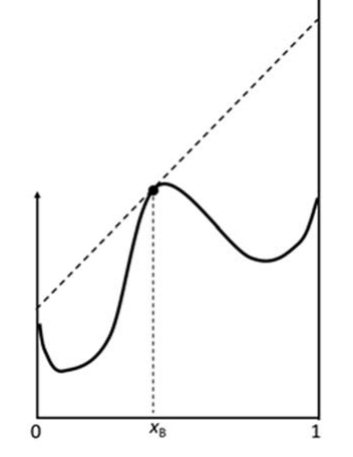
\includegraphics[scale=0.5]{melange.png}
    \end{figure}
    $\square$ $\mu_B<\mu^B$; $\square$ $\mu^A < \mu^B$; $\square$ $\mu_A < \mu_B$;
    $\square$ $\mu_A > \mu^A $; $\square$ $\omega >0$

    \item Quel est le lien entre la vitesse la plus probable $c_p$ et la vitesse quadratique moyenne $\sqrt{\bar{c^2}}$ d'une distribution de vitesse de Maxwell - Boltzmann? $c_p$ = ...

    $\square$ $\sqrt{\frac{2}{3}\bar{c^2}}$; $\square$ $\sqrt{\bar{c^2}}$; $\square$ $\sqrt{\frac{3}{2}\bar{c^2}}$; $\square$ $\frac{3}{2} \sqrt{\bar{c^2}}$; $\square$ $\frac{2}{3}\sqrt{\bar{c^2}}$

    \item Pour caractériser le compresseur d'un turbo, vous disposez des données suivantes : puissance de \SI{5}{kW} et débit d'air de \SI{80}{g/s}. Quelle est la pression absolue à l'admission du moteur, c'est-à-dire après la compression, si la température ambiante est de 25°C et la pression ambiante de 1 $bar$ ? (hypothèse: transformation réversible)

    $\square$ 2.18; $\square$ 1.52; $\square$ 1.96; $\square$ 2.86; $\square$ 1.37
\end{enumerate}

\nosolution

\end{document}
